\begin{questions}
  \question Напишете най-характерното за работата на един комутатор
  (\foreignlanguage{english}{switch}).

  \question Напишете най-малко три разлики между комутатор и маршрутизатор.

  \question Опишете поведението на маршрутизатор в режим на динамична размяна на
  маршрути.

  \question Каква е същността на оптимизацията за RIP "`Poison Reverse"'? Защо
  се налага имплементирането ѝ?

  \question Опишете IP адресите на интерфейсите и съдържанието на маршрутните
  таблици на трите маршрутизатора, ако те са конфигурирани така, че да има
  двупосочна комуникация между PC 1 и PC 2.

  \begin{center}
    \begin{tikzpicture}[
      align=center,node distance=2cm,
      start chain=going right,
      diagram item/.style={
        on chain,
        join
      }
      ]

      \node [
      diagram item,
      label=above:Router 1,label=267:eth0,label=-15:eth1
      ] {\includegraphics{router}};

      \node [
      start branch=1 going below left,
      diagram item,
      label=below:PC 1,label=30:eth0
      ] {\includegraphics{pc}};

      \node [
      diagram item,
      label=above:Router 2,label=-165:eth1,label=-15:eth0
      ] {\includegraphics{router}};

      \node [
      diagram item,
      label=above:Router 3,label=-165:eth0,label=273:eth1
      ] {\includegraphics{router}};

      \node [
      start branch=1 going below right,
      diagram item,
      label=below:PC 2,label=150:eth0
      ] {\includegraphics{pc}};

    \end{tikzpicture}
  \end{center}

  \question Дайте примери за IGP и EGP протоколи за маршрутизация. Напишете
  кратко пояснение за всеки пример.

  \question Какво наричаме мрежова маска?

  \question Опишете три недостатъка на NAT.

  \question Напишете броя валидни IP адреси за следните IPv4 мрежови маски:
  \begin{itemize}
    \item \texttt{/25}
    \item \texttt{/20}
    \item \texttt{/19}
    \item \texttt{/17}
  \end{itemize}

  \question Имаме мрежа с 500 хоста. Изберете мрежова маска, която осигурява
  най-малкото адресно пространство, в което те могат да се съберат.

  \question Обяснете в какво се състои тристранното ръкостискане
  (\foreignlanguage{english}{three-way handshake}) при TCP.

  \question Имате Linux-базирана система с един Ethernet интерфейс, на който е
  зададен IP адресът \texttt{192.168.0.2/255.255.255.240}. До какво ще доведе
  изпълнението на командата \texttt{route add -net 10.0.0.0 netmask 255.240.0.0
    gw 192.168.0.16}?

  \question Ако имаме мрежата \texttt{192.168.1.0/24}, на колко подмрежи ще бъде
  разделена тя, с помощта на маска с дължина \texttt{/26}?

  \question Посочете адресите за разпръскване
  (\foreignlanguage{english}{broadcast addresses}) на всяка подмрежа от
  предишния въпрос.

  \question Каква е целта на полето \texttt{time-to-live} в хедъра на IP?

  \question Каква е функционалността на маршрута по премълчаване
  (\foreignlanguage{english}{default route})?

  \question Вярно ли е, че тъй като TCP не може да разчита на IP да форматира
  пакетите правилно, IP адресът на дестинацията трябва да бъде включен в TCP
  хедъра?

  \question Какво наричаме автономна система
  (\foreignlanguage{english}{autonomous system, AS})?

  \question Какво разпръсква в мрежата маршрутизатор, който е конфигуриран да
  разчита на \foreignlanguage{english}{link-state} протокол за маршрутизация? А
  ако е конфигуриран с \foreignlanguage{english}{distance-vector} протокол за
  маршрутизация?

  \question[7] На графиката отдолу са изобразени четири маршрутизатора, които са
  конфигурирани за динамична маршрутизация с RIP. Ако не са имплементирани
  оптимизации за алгоритъма на RIP, какво ще бъде разстоянието между A и
  D след една стъпка от схождането на мрежата. (Приемете, че маршрутизаторите са
  били изключени до този момент)

  \begin{center}
    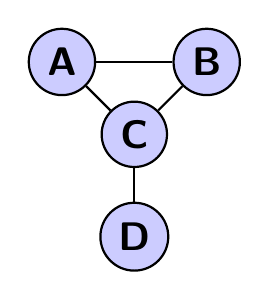
\begin{tikzpicture}[auto,node distance=1.3cm,
      thick,main node/.style={circle,fill=blue!20,draw,font=\sffamily\Large\bfseries}]


      \node[main node] (3) {C};
      \node[main node] (1) [above left of=3] {A};
      \node[main node] (2) [above right of=3] {B};
      \node[main node] (4) [below of=3] {D};


      \path[every node/.style={font=\sffamily\small}]
        (1) edge node {} (3)
            edge node {} (2)
        (2) edge node {} (3)
        (3) edge node {} (4);
    \end{tikzpicture}
  \end{center}
\end{questions}

%%% Local Variables:
%%% mode: latex
%%% TeX-master: "test"
%%% ispell-dictionary: "bulgarian"
%%% TeX-PDF-mode: t
%%% End:
